\documentclass[a4paper,11pt]{article}

% set up sensible margins (same as for cssethesis)
\usepackage[paper=a4paper,left=30mm,right=30mm,top=25mm,bottom=25mm]{geometry}
\usepackage{natbib} % Use the natbib bibliography and citation package
\usepackage{setspace} % This is used in the title page
\usepackage{graphicx} % This is used to load the crest in the title page
\usepackage{physics} % Used for \abs

% non-template packages
\usepackage{paralist}
\usepackage{multicol}
\usepackage{caption}
\usepackage{tabularx, booktabs}
\newcolumntype{Y}{>{\centering\arraybackslash}X}
\usepackage{listings}
\lstset{
	numbers=left, 
	numberstyle=\small, 
	numbersep=8pt, 
	frame = single, 
	language=Python, 
	framexleftmargin=17pt}

\usepackage{tikz}
\usepackage{smartdiagram}

\usepackage[font={small,it}]{caption}
\usepackage{hyperref}
\usepackage{xcolor}
\usepackage{lscape}
\hypersetup{
	colorlinks,
	linkcolor=teal,
	citecolor=teal,
	urlcolor=blue
}

\usepackage[english]{babel}
\usepackage{blindtext}
\usepackage{footnote}
\makesavenoteenv{tabular}
\makesavenoteenv{table}

%tikz stuff
\usepackage{tikz}
\usetikzlibrary{shapes, arrows, trees}
\tikzstyle{decision} = [diamond, draw, fill=green!20, text width=4.5em, text badly centered, node distance=3cm, inner sep=0pt]
\tikzstyle{block} = [rectangle, draw, fill=yellow!20, text width=3cm, text centered, rounded corners, minimum height=4em]
\tikzstyle{line} = [draw, -latex']
\tikzstyle{straight} = [draw]


\usepackage{array}
\newcolumntype{L}[1]{>{\raggedright\let\newline\\\arraybackslash\hspace{0pt}}m{#1}}
\newcolumntype{C}[1]{>{\centering\let\newline\\\arraybackslash\hspace{0pt}}m{#1}}
\newcolumntype{R}[1]{>{\raggedleft\let\newline\\\arraybackslash\hspace{0pt}}m{#1}}

\usepackage{float}

%\hypersetup{
%	colorlinks,
%	linkcolor={red!50!black},
%	citecolor={blue!50!black},
%	urlcolor={blue!80!black}
%}

\begin{document}
	
% Set up a title page
\thispagestyle{empty} % no page number on very first page
% Use roman numerals for page numbers initially
\renewcommand{\thepage}{\roman{page}}

\begin{spacing}{1.5}
	\begin{center}
		{\Large \bfseries
			School of Computer Science (BICA) \\
			Monash University}
		
		
		\vspace*{30mm}
		
		
\includegraphics[width=5cm]{graphics/MonashCrest.pdf}
		
		\vspace*{15mm}
		
		{\large \bfseries
			Literature Review, 2017
		}
		
		\vspace*{10mm}
		
		{\LARGE \bfseries
			Review of optimal multi-agent Pathfinding algorithms and usage in warehouse automation
		}
		
		\vspace*{20mm}
		
		{\large \bfseries
			Phillip Wong
			
			\vspace*{20mm}
			
			
			Supervisors: \parbox[t]{50mm}{Daniel Harabor,\\Pierre Le Bodic}
		}
		
	\end{center}
\end{spacing}

\newpage

\tableofcontents

\newpage
% Now reset page number counter,and switch to arabic numerals for remaining
% page numbers 
\setcounter{page}{1}
\renewcommand{\thepage}{\arabic{page}}

\section{Introduction}
The order picking process is the number one expense in the operating cost of warehouse systems \cite{de2007design}. 
% What
This project looks at the use of multi-agent pathfinding (MAPF) within warehouse automation. In particular we will we will be exploring Kiva systems, whereby the order-picking process is performed by automated vehicles. More detail about Kiva systems is provided in Section~\ref{sec:background}. Our work looks at finding an optimal solution multi-agent pathfinding.
% How
In order to find an optimal solution we will be using formulating the MAPF problem as a mixed integer program. Section~\ref{sec:optimal} will look at past approaches taken to MAPF.
% Why
The results of this literature review will help identify how we should position storage and picking stations in a warehouse. Additionally, we will be looking at developing a MAPF method which uses a pre-computed path oracle.

\section{Background} \label{sec:background}
In this project, we look at Kiva Systems (now known as Amazon Robotics). In Kiva systems, products are stored in mobile shelves known as storage pods. Robots known as drive units are responsible for retrieving and delivering storage pods to picking stations. A human worker is stationed at each picking station who picks the item off the pod before processing it (Figure~\ref{fig:kivaprocess}). Once the pod has been processed, the drive unit will return the pod
to an appropriate location in the warehouse.

\begin{figure}[h!]
	\centering
	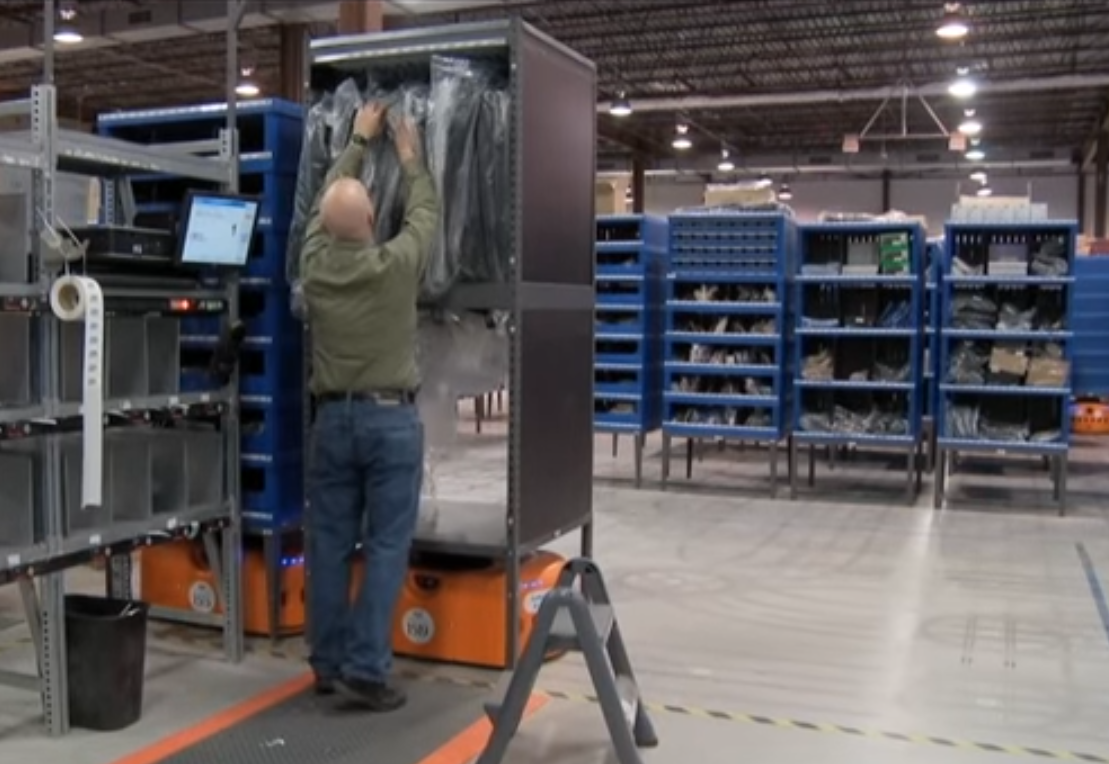
\includegraphics[width=0.6\textwidth ]{graphics/kivaprocess}
	\caption{A worker picking an order from a storage pod. The orange robot underneath is the drive unit. (\cite{kivayoutube2010quietlogistics})}
	\label{fig:kivaprocess}
\end{figure}


\noindent \textbf{Single-agent pathfinding}. Single-agent pathfinding aims to find a path from start node to goal node. A detailed review of single agent search algorithms can be found in the \textit{grid-based path planning competition} (\cite{sturtevant2015grid}). The paper overviews the entries to the competition and their relative performance. The algorithms are run on a number of game maps which are used for benchmarking \cite{sturtevant2012benchmarks}. While these results are a few years old, we are expecting to new approaches from this year's GPPC (2017).

In this project, we aim to look at two single-agent search algorithms: \textit{jump point search} and \textit{compressed path databases}. The authors of Jump Point Search and Compressed Databases provide an overview of a large number of search algorithms (\cite{botea2013pathfinding}). In it they outline these algorithms and techniques in the context of computer games. cover heuristics, symmetry elimination which is the core of Jump Point Search. and specific gaps in the literature between video games.

%\subsection{Jump Point Search}
%Jump point search
%
%\subsection{Compressed Path Databases}
%Compressed path databases
%\cite{strasser2015compressing}


\noindent \textbf{Multi-agent pathfinding}. Solving MAPF optimally is an NP-hard problem (\cite{yu2013structure}). As a result, Kiva systems are generally looked at with suboptimal algorithms with scalability in mind. Here we are focusing on an optimal approach, while it is not scalable to the desired size (1000+ agents), we will be looking at making a trade-off between speed and solution quality by creating bounded-suboptimal algorithm.

%Take a MAPF problem instance where we have $k$ agents on a graph with $n$ nodes.
%Within MAPF, we are focusing on an optimal solution. The following sections will focus on optimal MAPF algorithms as well as suboptimal variants of these algorithms. More about optimal MAPF is described in Section~\ref{sec:optimal}.

\noindent \textbf{Bounded-suboptimal varient}. A \textit{bounded suboptimal variant} is a variant of an optimal MAPF algorithm. The defining feature of a bounded suboptimal variant is that we can guarantee that the cost of the solution, $B$ lies within the optimal cost $C$ and $w*C$ where $w$ is a user-defined parameter. Hence:

\[C \le B \le w*C\]

Our project is aiming to make a bounded suboptimal variant of our algorithm due to the large-scale of the simulation (Section~\ref{sec:background}). By adjusting $w$ we are able to relax the problem and find a solution faster at the loss of solution quality.

\section{Problem definition}
This section will formally define the MAPF problem in the context of Kiva Systems. The goal of MAPF is to find a path for each agent to their goal while ensuring that no path conflicts. 

\begin{itemize}
	\item A path is a list of action $a$ at timestep $t$ where $a \in \{up, down, left, right, wait\}$
	\item A path is said to conflict with another when on the same timestep: two agents share the same node or the agents cross the same edge.
\end{itemize}

In order to reduce the complexity of the MAPF algorithm, the environment of a Kiva systems is modeled as a square grid map (Figure~\ref{fig:kivawarehouse}). On this map we have $k$ drive unit agents.

\begin{itemize}
	\item Graph $G(V, E)$ where $V$ is the set of nodes on the grid map and $E$ is the set of edges between nodes.
	\item A set of agents, $K$, where for all $k \in K$, $location(k) \in V$ and $goal(k) \in V$
\end{itemize}

Each action 

\begin{figure}[h]
	\centering
	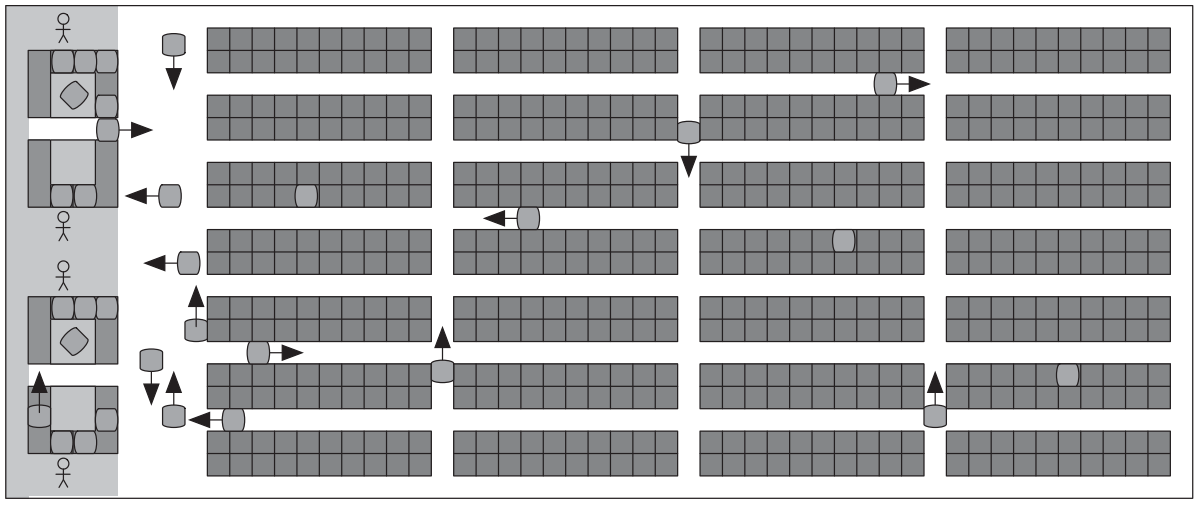
\includegraphics[width=0.9\textwidth]{graphics/kivasystemlayout}
	\caption{Kiva system represented on an orthagonal grid map (\cite{wurman2008coordinating})}
	\label{fig:kivawarehouse}
\end{figure}


%\section{Single-agent pathfinding}


\section{Suboptimal multi-agent pathfinding algorithms}
Suboptimal MAPF algorithms usually use a decentralized approach\footnote{decentralized is also known as decoupled}. In a decoupled approach, paths are found for one agent at time as oppose to a coupled approach which looks at all agents globally. These algorithms usually have the properties of being suboptimal and incomplete.

%\begin{center}
%\begin{tikzpicture}
%\centering
%\draw[step=1cm,gray,very thin] (0,0) grid (5,3);
%\fill[gray!] (0,0) rectangle (3,1);
%\node at (0.5, 2.5) {$a_2$};
%\node at (0.5, 1.5) {$a_1$};
%\end{tikzpicture}
%\end{center}

\subsection{Cooperative A*}
Cooperative A*
Exponential in number of agents

\cite{holte1995hierarchical}

\cite{silver2005cooperative} gives an overview of these three algorithms.

\subsection{FAR}
Flow Annotation Replanning (FAR) (Wang and Botea 2008) imposes unidirectional travel on top of an initially undirected gridmap. The travel direction alternates across the rows (and columns), covering the grid with criss- crossing virtual “road lanes”. Topology-specific additional rules, applied locally, preserve the connectivity across the map. In terms of map abstraction, this boils down to remov- ing some directed edges from a graph, as opposed to splitting a map into subgraphs. FAR computes a path for each unit independently, in a unit-centric decomposition. Conflicts, such as cycles, are addressed at runtime. A common idea with our work is restricting the traffic flow by ignoring some edges and imposing a travel direction on others. The flowin- side SDP high-contention areas is restricted as shown later in this paper. We take advantage of the specific topology of high-contention areas, ensuring that they are free from local deadlocks

\subsection{MAPP}
MAPP (\cite{wang2011mapp}) is a suboptimal algorithm which main benefit is its polynomial runtime complexity of $O(n^2k^2)$ where $n$ is the number of nodes on the graph and $k$ is the number of agents. It guarantees this by identifying sets of units which are guaranteed to run in polynomial time and is complete for slidable problems if there exists an $\Omega$ path for each agent (Figure~\ref{fig:omegapath}).

% MAPP that it does not require replanning.

\begin{figure}[H]
	\centering
	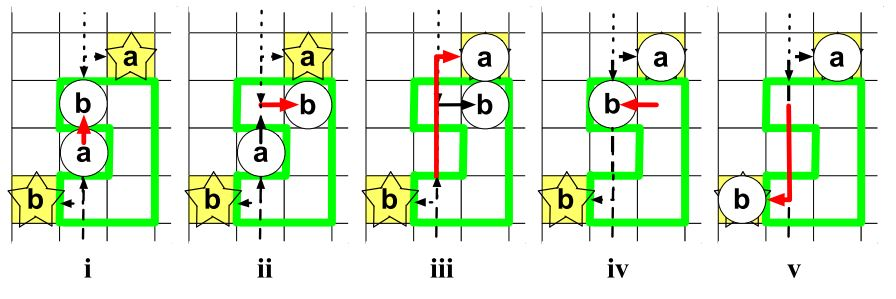
\includegraphics[width=\linewidth]{graphics/mappblank}
	\label{fig:mappblank}
	\caption{Example of how MAPP works (\cite{wang2011mapp})}
\end{figure}

In comparison to FAR and WHCA*, MAPP excels in having high completeness at 92\%--99.7\%, compared to FAR (81.87\%) and WHCA* (80.87\%). Speed-wise, MAPP is comparable to WHCA* and 10 times slower than FAR  but in scenarios where MAPP has $\Omega$ paths, MAPP is 2.18 times slower than FAR and 4.8--5.2 times faster than WHCA*.



\begin{figure}[H]
	\centering
	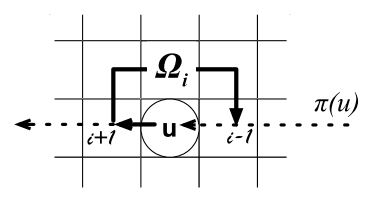
\includegraphics[width=0.4\linewidth]{graphics/omegapath}
	\label{fig:omegapath}
	\caption{An example of an alternate path, $\Omega$ (\cite{wang2011mapp})}
\end{figure}


\section{Optimal multi-agent pathfinding algorithms} \label{sec:optimal}
Optimal MAPF algorithms usually use a coupled approach also known as centralized approach. A coupled approach finds paths for all agents at once. 




Here we look at multi-agent pathfinding algorithms which aim to find the optimal solution based on some objective function. The objective function will be noted per algorithm. Our main aim is to determine the benefits and downsides of each algorithm.


Coupled approach: All agents at one! A* ICTS

\cite{krontiris2013feasibility} looked at the feasibility.

\subsection{Centralized A*}
Centralized A* is exponential in the number of agents $O(n^k)$

There are a number of algorithms based on Centralized A*, 

One variant of is an algorithm called enhanced partial A* expansion (EPEA*). The original algorithm \cite{yoshizumi2000partial}. An improvement on PEA* is EPEA* (\cite{felner2012partial}, \cite{goldenberg2014enhanced}).

Another variant is M*.

Independence Detection and Operator Decomposition provides an exponential speed up to Centralized A* as it reduces the number of agents being processed, more details about ID in Section~\ref{sec:od} and OD in Section~\ref{sec:od}.

\cite{ferner2013odrm} improves on M* by applying operator decomposition.

\subsection{Conflict based search}
The conflict-based search algorithm (\cite{sharon2015conflict}) relies on building a binary tree known as a  \textit{constraint tree} (CT). Each node in the CT describes a set of constraints, a solution and the cost of this solution. A constraint prohibits an agent $a$ from being at node $n$ at timestep $t$, in the form of $\langle a, n, t \rangle$.

A node in the CT is processed by finding the shortest path for each agent to their goal making sure to satisfy the constraints described by the node. If this path is not valid and a collision has occurred between two agents: $a_1, a_2$ then CBS branches and adds two successor nodes. Both successor nodes inherit the constraints of the parent node. Additionally the left successor will adds a new constraint $\langle a_1, n, t \rangle$ while the right node will add the constraint $\langle a_2, n, t \rangle$. CBS is optimal as it chooses the node to expand searching the constraint tree for the node with the lowest cost.

As CBS branches at every conflict, it is exponential in the number of conflicts. In comparison to EPEA*, CBS performed worse in maps with open spaces where sets of agents may be \textit{strongly coupled}, that is they frequent have a high rate of path conflicts between one another. On the other hand CBS was found to perform better in maps with bottlenecks, where A* would 


CBS is exponential in the number of conflicts In comparison to ICTS and A* CBS was found to be best in maps with bottlenecks (Fig.~\ref{cbsresults1}).

A bounded-suboptimal variant of CBS, ECBS features \cite{barer2014suboptimal} \textbf{TODO} Recently iECBS expanded on this with the use of highways and  \cite{cohen2016improved}.

\begin{figure}[!htb]
	\centering \tiny
	\begin{minipage}{0.4\textwidth}
	\centering
	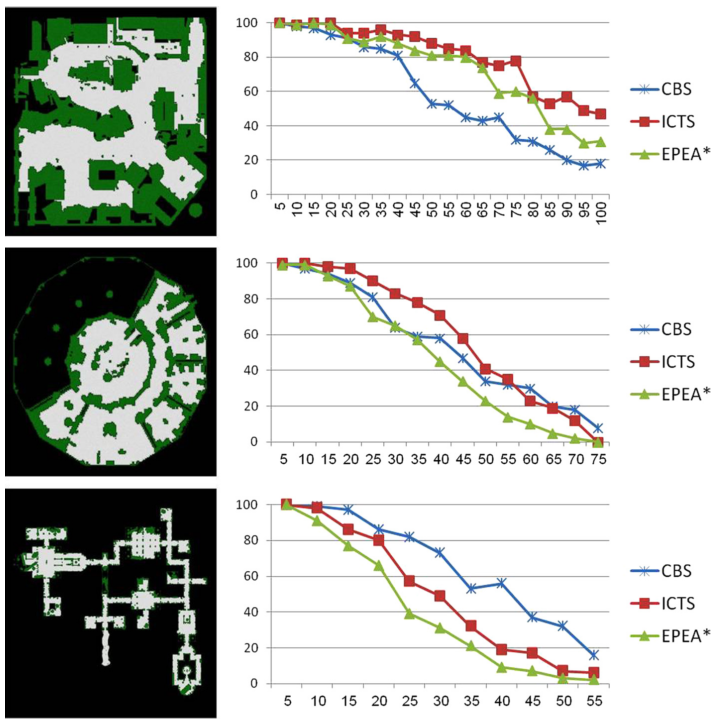
\includegraphics[width=\linewidth]{graphics/cbsresults1}
	\caption{A Small Region of a Kiva Layout (\cite{sharon2015conflict}). Picking stations located on the left and storage pods laid out in rows.}
	\label{cbsresults1}
	\end{minipage}
	\begin{minipage}{0.4\linewidth}
		\centering
	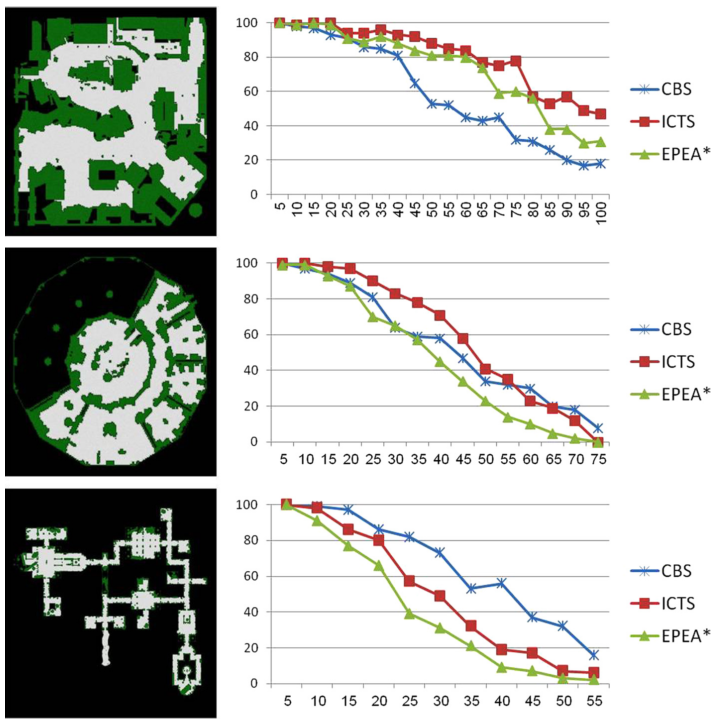
\includegraphics[width=\linewidth]{graphics/cbsresults1}
	\caption{A Small Region of a Kiva Layout (\cite{sharon2015conflict}). Picking stations located on the left and storage pods laid out in rows.}
	\label{cbsresults2}
	\end{minipage}
\end{figure}

Here CBS was compared against ICTS, EPEA*.

\subsection{Increasing Cost Search Tree}
This section describes the Increasing Cost Search Tree (ICTS) an optimal, complete MAPF algorithm (\cite{sharon2011increasing}). The ICTS algorithm generates a tree known as an \textit{increasing cost tree} (Figure~\ref{fig:increasingcosttree}). Each node in the tree describes a cost $C$ for each agent $[C_1,\dots,C_k]$. ICTS finds a valid solution when every agent $a_i$ is conflict-free and it generates these paths based off the cost described in the node by exploring all paths which are equal to $C_i$.  To build the tree, the root starts containing the an optimal cost disregarding any conflicts for each agent. When it does not find a valid solution, the algorithm will branch and generate $k$ successors, one for each agents. In each of the successors, the cost of $i$ will increment e.g. for successor 2: $[C_1,C_{2}+1,\dots,C_k]$. By exploring the tree in breadth-first manner, ICTS ends up with an optimal solution.

\begin{figure}[!htb]
	\centering
	\centering
	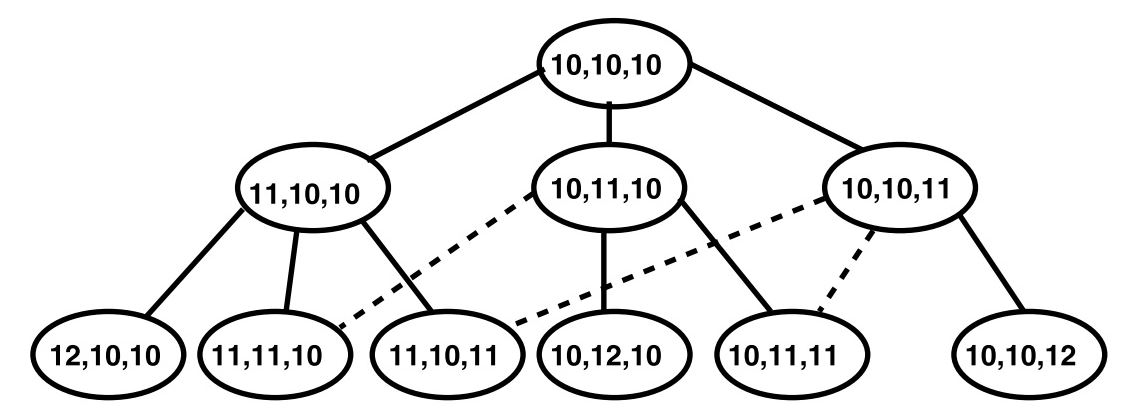
\includegraphics[width=0.9\linewidth]{graphics/ictstree}
	\caption{ICT for three agents (\cite{sharon2011increasing})}
	\label{fig:increasingcosttree}
\end{figure}

The ICT grows exponentially in $\Delta$, where delta is the difference between the optimal collision-free cost and the optimal cost which ignores collision (the root node). Hence the downfall of ICTS is an environment with many conflicts occurs or it is costly to resolve the conflicts, thus having a large $\Delta$. In comparison to $A*$ which is exponential in $k$, ICTS is exponential in $\Delta$ so it benefits most on open maps with many agents.

\subsection{Integer Linear Programming}
Integer Linear Programming (ILP) is an optimization technique. It looks at an objective function subject to a list of constraints and finds the optimal solution for each variable.

\cite{ma2016optimal} reduction to the integer multi- commodity flow problem on a time-expanded network.

\cite{yu2016optimal} takes a Network Flow approach. The solver uses the branch-and-bound algorithm. Anytime approach.


\cite{yu2013multi} connects multi-agent path planning on graphs (roadmaps) to network flow problems, showing that the former can be reduced to the latter, therefore enabling the application of combinatorial network flow algorithms, as well as general linear program techniques, to multiagent path planning problems on graphs.

\cite{yu2016optimal} looks at Complete Algorithms and Effective Heuristics.

\cite{yu2015optimal} looks at the Structure and Computational Complexity.


\section{Independence detection and Operator decomposition}
Here we describe any techniques which may be applied to most MAPF algorithms and cause a speedup.

\subsection{Independence detection} \label{sec:id}
\cite{standley2010finding} Independence detection (ID) allowed the paths of groups of agents to be computed independently, without sacrificing optimality 

\textbf{Standley (Standley 2010) presented (= ?V independence detection (ID) framework. ID partitions
the problem into smaller independent subproblems, if possi- ble, and solves each problem separately. Standley also intro- duced operator decomposition (OD) which considers mov- ing a single agent at a time. OD reduces the branching fac- tor at the cost of increasing the depth of the solution in the search tree.}

\subsection{Operator decomposition} \label{sec:od}
\cite{standley2010finding} Operator decomposition (OD) is used to reduce the branching factor of the MAPF algorithms.

\section{Discussion}
There are a number of algorithms which have been developed in

We should study these algorithm in the warehouse environment. Besides CBS and ILP (TAPF), other algorithms have not been compared against one another. Our research focuses on the area of ILP

\begin{table}
\centering
\small
\begin{tabular}{ l c c c c c p{2.3cm} }
	\textbf{Name} & \textbf{BSO}\footnote{BSO: whether the algorithm has a bounded-suboptimal variant}  & \textbf{Complete} & \textbf{Complexity\footnote{Complexity: runtime complexity}} & \textbf{SQ\footnote{SQ: solution quality}} & \textbf{KS}\footnote{KS: whether the algorithm was tested in a Kiva System environment} & \textbf{Comparison}\footnote{Comparison: other MAPF algorithms used for benchmark comparison} \\
	\hline
	\multicolumn{7}{l}{\textbf{Optimal}} \\
	\hline
	CBS 				& N & Y & Exp conflicts & Opt & Y & ICTS, EPEA* \\
	Centralized A* 		& Y & Y & Exp agents & Opt & N & ??? \\
	ICTS 				& Y & Y & Exp $\Delta$ & Opt & N & A*, A*+OD \\
	ILP	(NF)			& Y & Y & Exp conflicts & Opt & Y & CBS \\
	ILP	(TAPF)			& Y & Y & Exp conflicts & Opt & Y & CBS \\
	\hline
	\multicolumn{7}{l}{\textbf{Suboptimal}} \\
	\hline
	FAR  				& N & N & Poly & Sub Opt & N & \\
	MAPP 				& Y & Y & Poly & Sub Opt & N & WHCA*, FAR \\
	WHCA* 				& N & N & Poly & Sub Opt & N & \\
	
	
\end{tabular}
\end{table}

\bibliographystyle{dcu}
\bibliography{bibliography}
	
\end{document}
